\documentclass[border=4pt]{standalone}
\usepackage{amsmath,amssymb,tikz}
\usetikzlibrary{arrows.meta,calc,matrix,positioning}
\definecolor{figB}{RGB}{31,90,166}\definecolor{figR}{RGB}{176,48,48}\definecolor{figG}{RGB}{46,125,50}\definecolor{figO}{RGB}{214,120,20}
\begin{document}
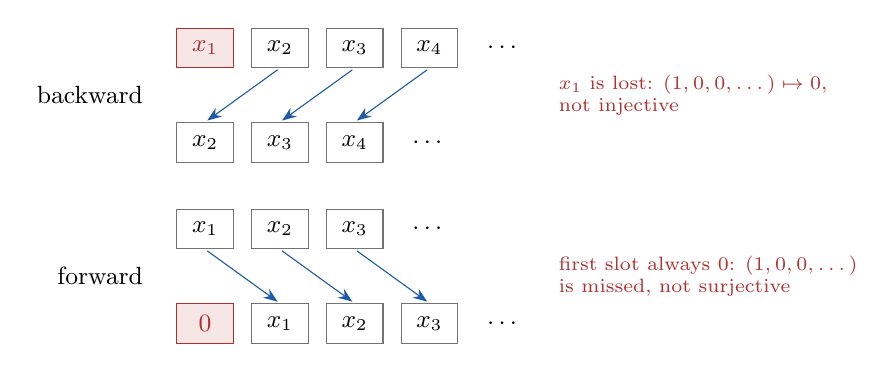
\begin{tikzpicture}[x=0.95cm,y=1cm,>={Stealth[length=1.8mm]},
  slot/.style={draw=black!55,minimum width=0.72cm,minimum height=0.5cm,inner sep=0pt,font=\small},
  lost/.style={slot,draw=figR,fill=figR!12,text=figR},
  mapsto/.style={->,figB,thin,shorten >=1pt,shorten <=1pt}]
% backward shift
\node[font=\small,anchor=east] at (-0.7,0.6) {backward};
\foreach \i in {1,2,3,4} \node[slot] (a\i) at (\i-1,1.2) {$x_{\i}$};
\node[font=\small] at (4,1.2) {$\cdots$};
\foreach \i/\j in {2/1,3/2,4/3} \node[slot] (b\j) at (\j-1,0) {$x_{\i}$};
\node[font=\small] at (3,0) {$\cdots$};
\node[lost] at (0,1.2) {$x_1$};
\foreach \i/\j in {2/1,3/2,4/3} \draw[mapsto] (a\i.south)--(b\j.north);
\node[font=\scriptsize,figR,anchor=west,align=left] at (4.6,0.6) {$x_1$ is lost: $(1,0,0,\dots)\mapsto 0$,\\ not injective};
% forward shift
\begin{scope}[yshift=-2.3cm]
\node[font=\small,anchor=east] at (-0.7,0.6) {forward};
\foreach \i in {1,2,3} \node[slot] (c\i) at (\i-1,1.2) {$x_{\i}$};
\node[font=\small] at (3,1.2) {$\cdots$};
\node[lost] (d0) at (0,0) {$0$};
\foreach \i/\j in {1/1,2/2,3/3} \node[slot] (d\j) at (\j,0) {$x_{\i}$};
\node[font=\small] at (4,0) {$\cdots$};
\foreach \i in {1,2,3} \draw[mapsto] (c\i.south)--(d\i.north);
\node[font=\scriptsize,figR,anchor=west,align=left] at (4.6,0.6) {first slot always $0$: $(1,0,0,\dots)$\\ is missed, not surjective};
\end{scope}
\end{tikzpicture}
\end{document}
